\section{ADDITIONAL EXPERIMENTS}\label{sec:add_expes}

\subsection{Details of \textsf{glmnet} versus \textsf{SLOPE} Comparison}
\label{sec:slope-vs-glmnet}

In this experiment, we ran the \pkg{glmnet}~\parencite{friedman2022} and \pkg{SLOPE}~\parencite{larsson2022d} packages on the \dataset{bcTCGA} dataset, selecting the regularization sequence \(\lambda\) such that there were 100 nonzero coefficients and clusters at the optimum for \pkg{glmnet} and \pkg{SLOPE} respectively.
We used a duality gap of \(10^{-6}\) as stopping criteria.
The features were centered by their means and scaled by their standard deviation.
The code is available in the supplement.

\subsection{Study on Proximal Gradient Descent Frequency}

\begin{figure*}[htb]
  \centering
  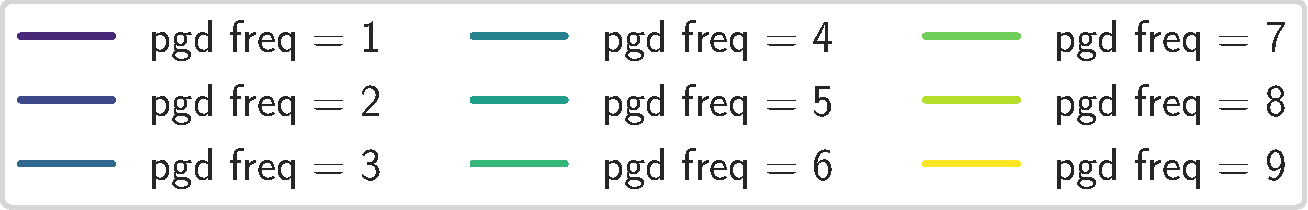
\includegraphics[scale=0.47]{pgd_freq_legend.pdf}
  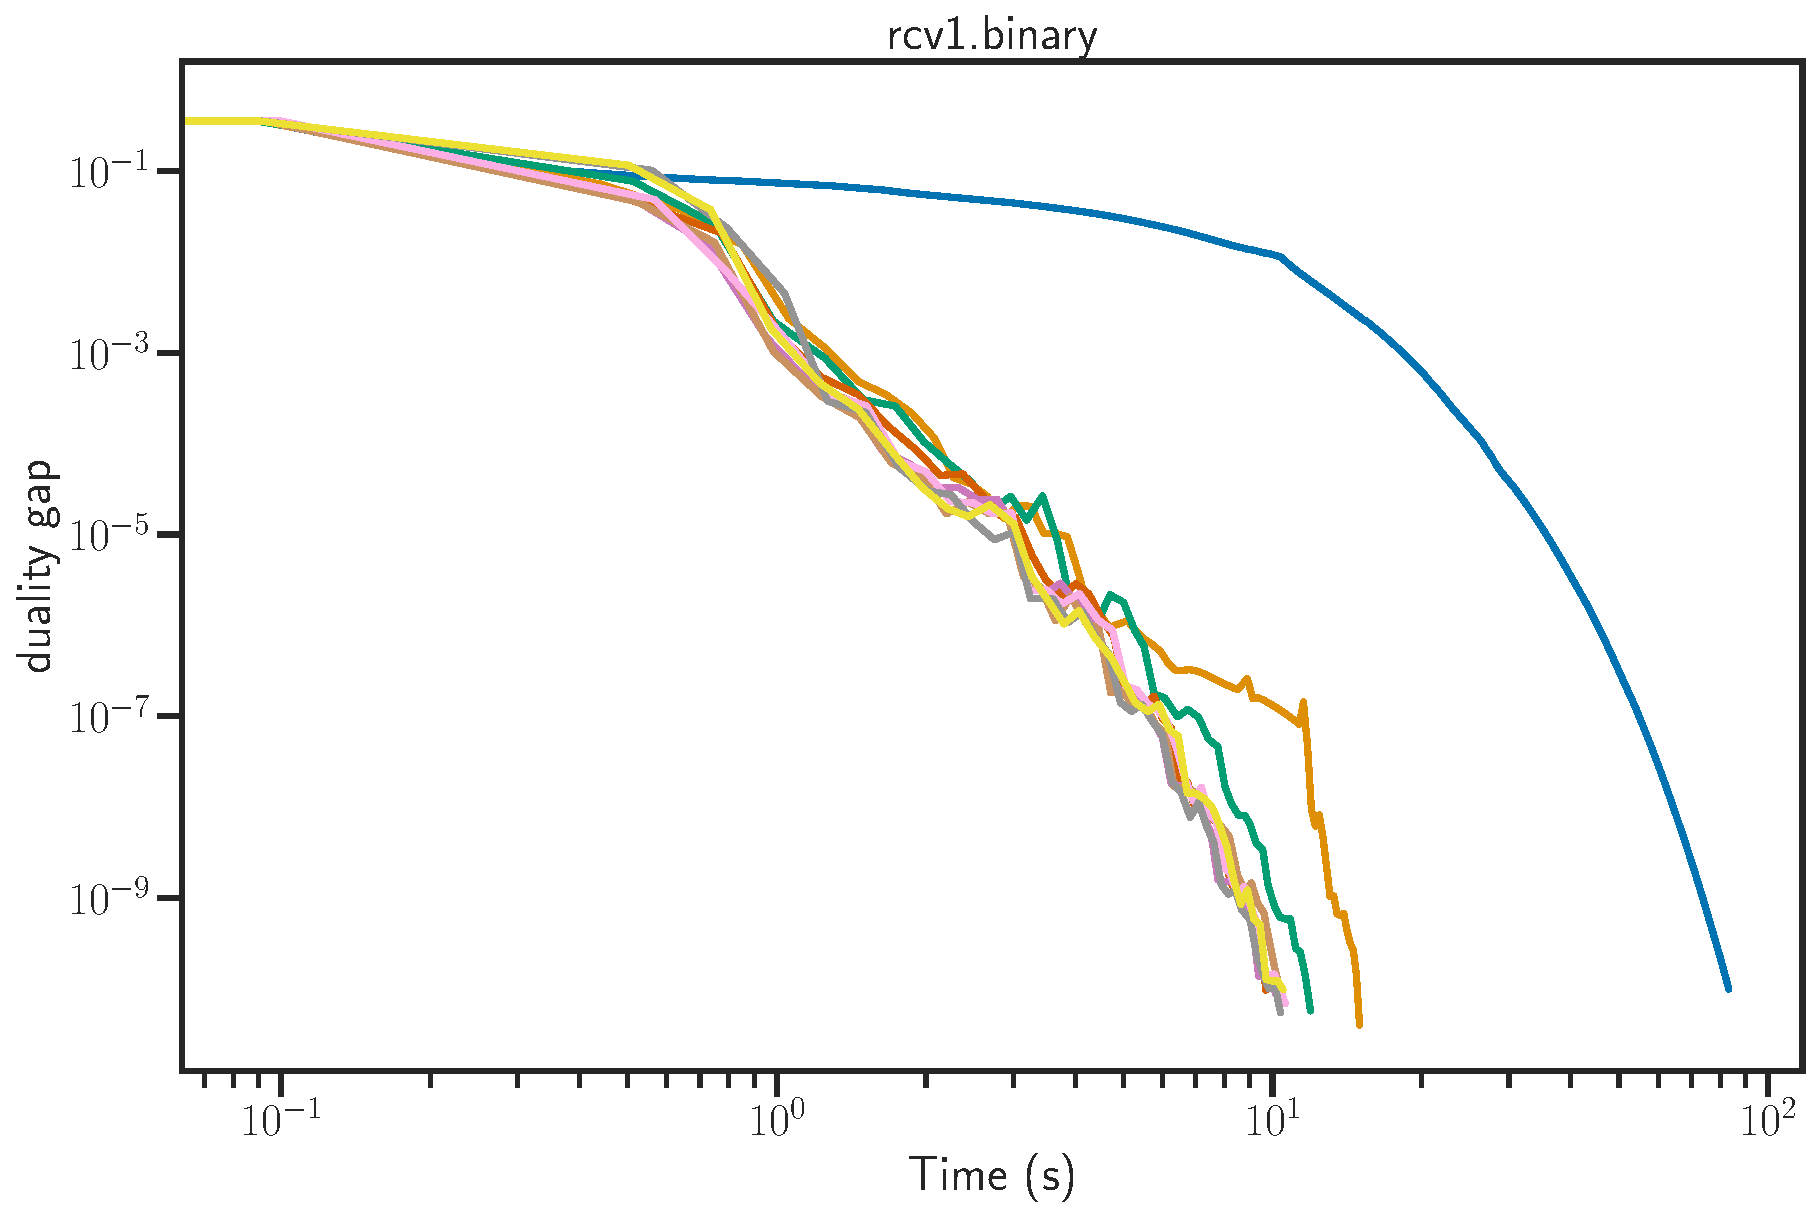
\includegraphics[scale=0.5]{pgd_freq_expes.pdf}
  \caption{Study on proximal gradient descent frequency.}
  \label{fig:pgd_freq}
\end{figure*}
